\chapter{Progress towards studies of quantum magnetism}
\label{ch:chap6}

A straightforward extension of the work presneted in this thesis would be to control interparticle spacing via an optical lattice. For these and additional experiments using quantum degenerate fermionic strontium we purchased and installed an optical lattice system. Our lattice is implemented using a Coherent Verdi V-18 which is shapped and propagated to our science chamber in free space. \hl{Fig} shows the optical path for each arm of our cubic lattice. 

Unfortunately, complications due to heating when loading the lattice has limited our success in this optical trap. I want to go over what we have been able to do so far with the lattice.

How did we characterize?
	Kaptiza-dirac extension
	
What convinced us we were having problems?

What are some ideas we could do in the lattice?
	Zeno
	faster cooling via stimulated raman potentailly? (can I model this somehow?)
	repulzively bound molecules?
	use interaction control in lattice with the zeno thing
	
\section{Optical lattice trap: 532\,nm} \label{ssec:532sys}
Until recently, experiments on the Neutral apparatus were confined to work with bulk gases in an optical dipole trap.
While optical dipole traps are useful for efficient evaporation and thermalization of an ultracold gas, optical lattices greatly extend our capabilities for studying ultracold molecules and novel many-body quantum states \hl{give some refs}.

Optical lattices are formed by a standing wave of light which creates a defect free periodic potential.
These traps are extremely versatile and have enabled the observation of the superfluid - Mott insulator transition \cite{Greiner2002}, artificial gauge fields for neutral atoms \cite{Lin2011}, quantum microscopy with single-site resolution \cite{Bakr2009}, and investigations of quantum magnetism \cite{Hart2015,Greif2015}. 
They are among the most well-established techniques for controlling a quantum state and have proven to be great tools for exploring the connection between few- and many-body systems \cite{Bloch2008}.

\subsubsection{Background} \label{sec:latBackground}
An optical lattice is created by counterpropagating two laser beams to form a standing wave pattern, which for two plane waves in one dimension results in a periodic potential given by 
	\begin{equation}
		 V(x) = V_{lat} \; \sin^2(k_L x)
	\end{equation}
where $V_{lat}$ is the lattice depth determined by the polarizability of the atom for a given trapping wavelength $\lambda$ and laser intensity $I$, and $k_L$ is the lattice wavevector.
This potential can be readily extended to three dimensions using two additional pairs of counterpropagating laser beams along the $y$ and $z$ directions which results in a 3D cubic lattice.
Depth of the trapping potential, $V_{lat}$, is controlled by varying the intensity of the lattice beams.

Periodic potentials are powerful because they break the translational invariance of space which results in the formation of band structure and the opening of bandgaps or disallowed particle energies \cite{Ashcroft1976}.
Because of this broken invariance, $p$ is no longer a good quantum number and must be replaced by two new quantum numbers: the band index, $n$, and the quasimomentum, $q$.
In one dimension, quasimomentum is specified by $q = p - nG$, where $G=2\pi/a$ is a reciprocal lattice vector, and $a$ is the real space lattice constant.
Fig.\;\ref{fig:bandStructure} shows how the band structure varies as the lattice depth is increased.
Optical lattices have a lattice spacing $a = \lambda /2$ which determines the reciprocal lattice vector $G = 4\pi / \lambda = 2 \hbar k_L$ and a natural energy scale $E_r = \frac{\hbar^2 k_L^2}{2m}$ where $m$ is the atomic mass and $k_L$ is the lattice wavevector, $k_L = 2\pi / \lambda$.
From the band structure, we see that the bandwidth of each band, given by $\Delta E = E_{q=\hbar k_L} - E_{q=0}$, decreases as the lattice depth is increased.
In the limit that $V_{lat}\!\rightarrow\!\infty$ the band structure reduces to a ladder of harmonic oscillator levels spaced by $\hbar \omega_{ho} = \sqrt{4 V_{lat} E_r}$.
Although, for moderately deep lattices, $V_{lat} \gtrsim 5\,$E$_r$, this approximation is valid near the center of the Brillioun zone, $q = 0$, and provides a simple form to estimate the energy gaps between bands \hl{\cite{Jaksch1998,Jaksch2005}.}
	\begin{figure} \label{fig:bandStructure}
		\centerline{
		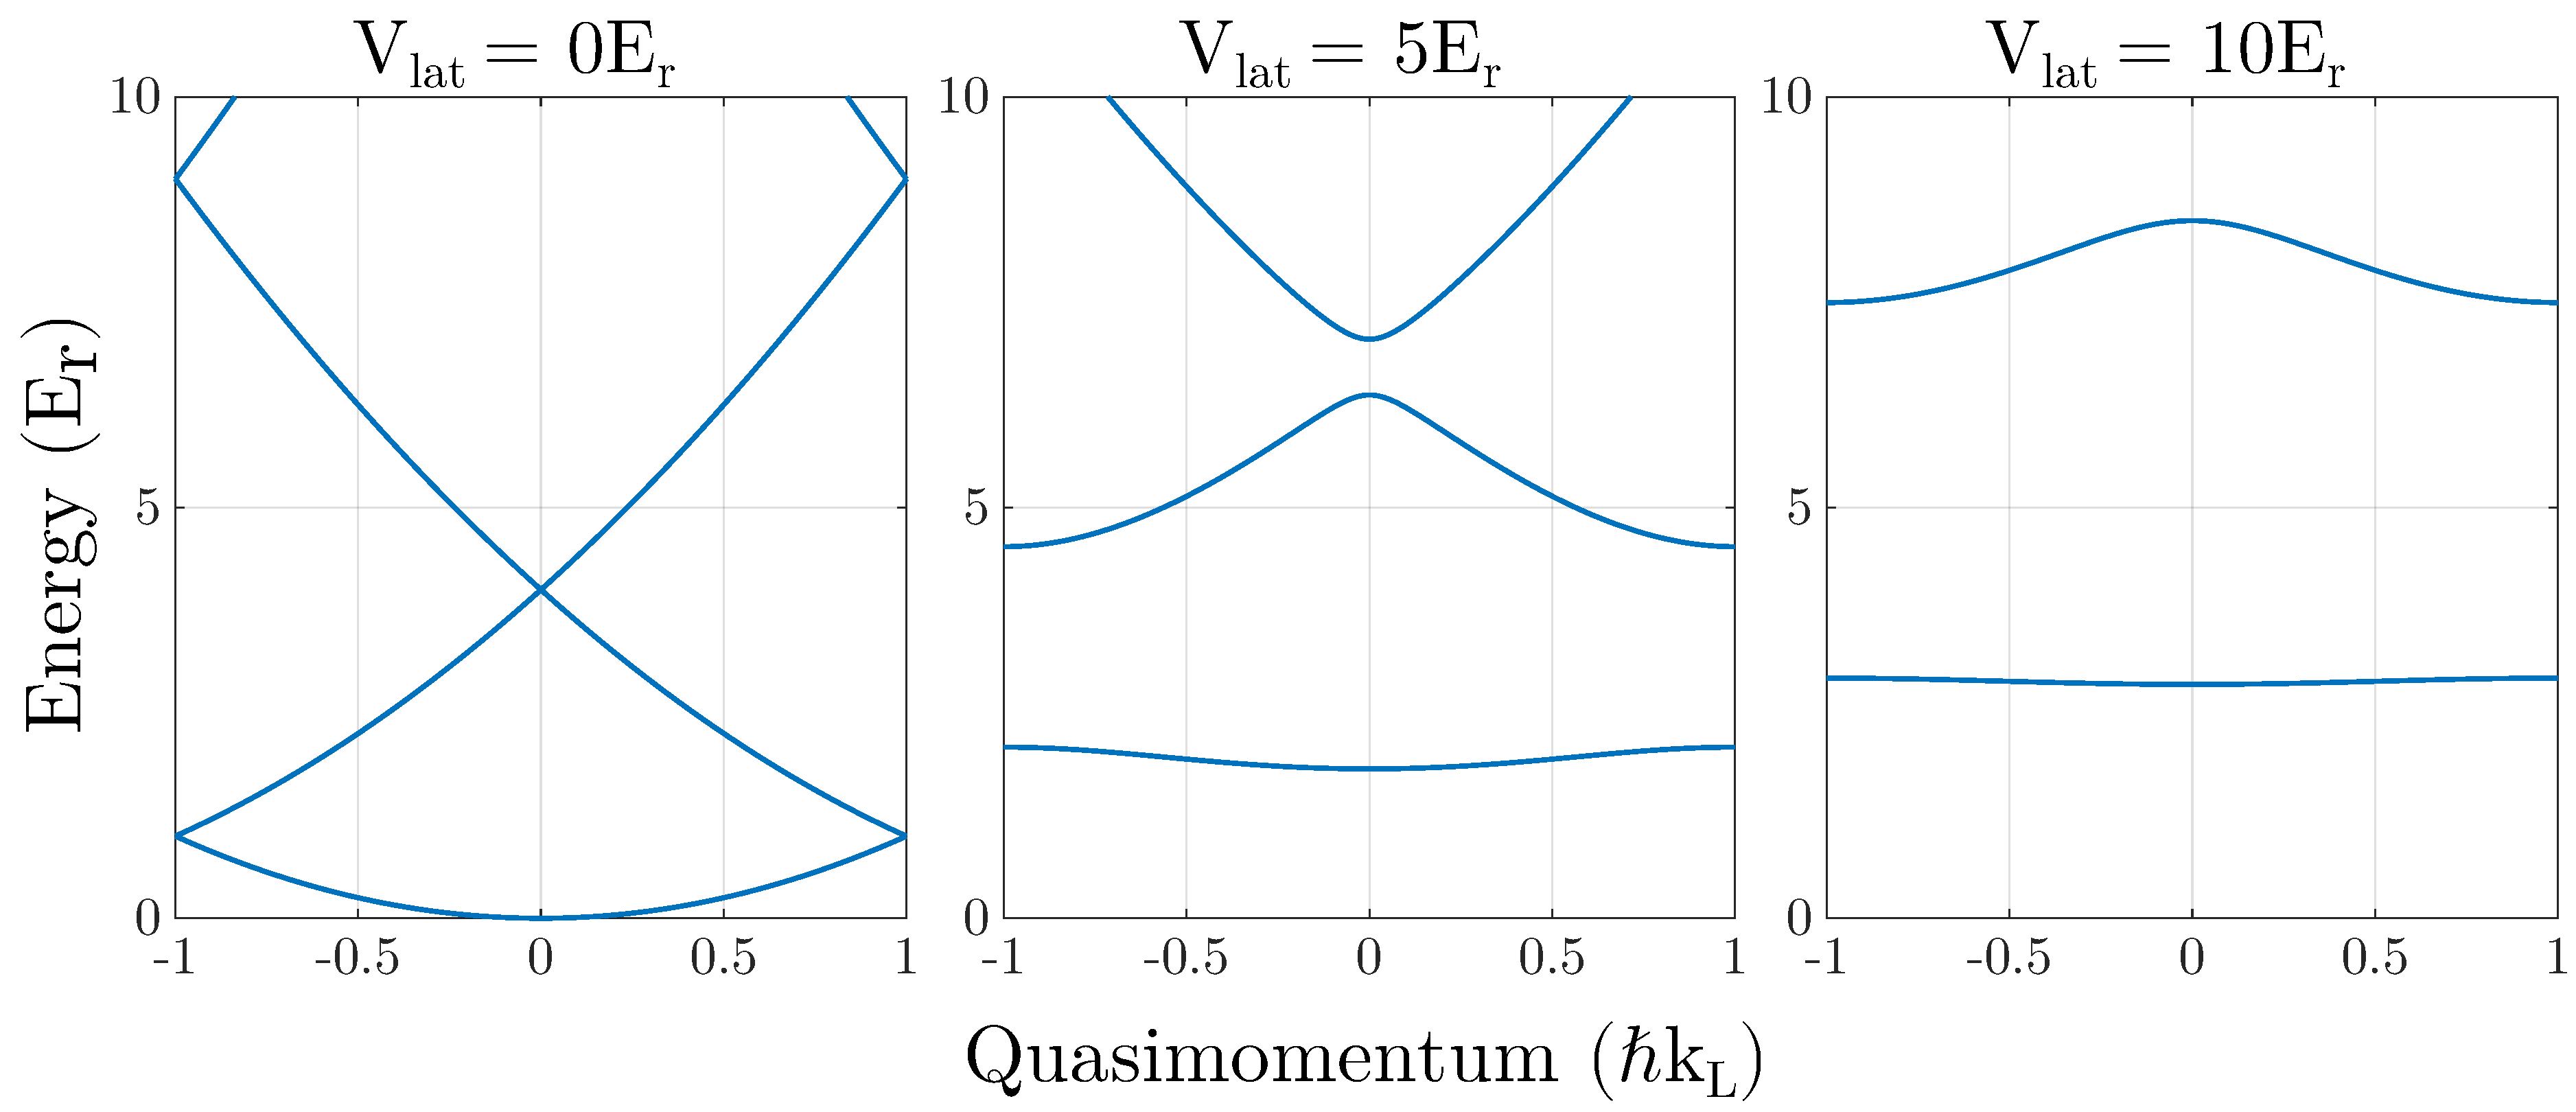
\includegraphics[width=\textwidth]{lattice_bandStructure.pdf}}
		\caption{1D band structure as a function of lattice depth}{One dimensional band structure for an optical lattice as the lattice depth is increased. The band energies are found by solving the Schr\"{o}dinger equation using the Bloch functions of Eq.\;\ref{eq:blochFunc}.}
	\end{figure}

Solutions to the Schr\"{o}dinger equation in a periodic potential are given by the Bloch functions \cite{Ashcroft1976}
	\begin{equation} \label{eq:blochFunc}
		 \phi_q^{(n)}(x) = e^{iqx/ \hbar} \; u_q^{(n)}(x)
	\end{equation}
These eigenstate wavefunctions are specified for a given quasimomentum $q$, and band index $n$. 
Their corresponding energy eigenvalues define the band structure of the lattice shown in Fig.\,\ref{fig:bandStructure}.
From Eq.\,\ref{eq:blochFunc} we see that the Bloch functions are the product of plane waves modulated by a function $u_q^{(n)}(x)$, which shares the periodicity of the underlying lattice potential \cite{Ashcroft1976}.
For an optical lattice this modulating function can be expanded in a basis of plane waves through a Fourier decomposition of the lattice potential in Eq.\,\ref{eq:1dlattice}, which gives \cite{Greiner2003},
	\begin{equation} \label{eq:blochMod}
		 u_q^{(n)}(x) = \sum_l c_l^{(n,q)} \; e^{i2lk_Lx}
	\end{equation}
Here $c_l^{(n,q)}$ are the coefficients for each plane wave in the basis expansion that are found by diagonalizing the lattice Hamiltonian \cite{Greiner2003}.

Often, we are interested in the dynamics of particles on a particular lattice site, but since Bloch functions are delocalized over the entire lattice, it is useful to instead use the Wannier functions. 
These functions provide an orthogonal and normalized set of wavefunctions that are maximally localized to a specific lattice site. 
The Wannier function for a localized particle in the n$^{th}$ band of a lattice site located at position x$_i$ is given by \cite{Jaksch2005}
	\begin{equation} \label{eq:wannier}
		 w_{n}(x - x_i) = \mathcal{N}^{-1/2} \sum_q e^{iqx_i/ \hbar} \; \phi_q^{(n)}(x)
	\end{equation}
where $\mathcal{N}$ is a normalization constant and $\phi_q^{(n)}(x)$ are the Bloch functions of Eq.\;\ref{eq:blochFunc}.
This localized description of particles allows us to calculate important physical quantities which govern dynamical properties of the lattice such as the tunneling rate, $J/ \hbar$, and on-site interaction energy, $U$. 
As $V_{lat}\!\rightarrow\!\infty$, the Wannier functions approach the eigenfunctions of the harmonic oscillator, which allows us to estimate the spatial extent of an atomic wavefunction by $a_{ho} = \sqrt{\frac{\hbar}{m \omega_{ho}}}$ \cite{Jaksch2005}.

\subsubsection{Setup and alignment} \label{sssec:532_align}
\paragraph{Setup}\label{ssec:lattice_setup}

Our optical lattice operates at $\lambda=532\,$nm and is derived from a Coherent Verdi V-18 single mode laser which is sent through separate AOMs for intensity control of each arm before propagating in free space to the atoms. 
We label these arms A, B, \& C as noted in Fig.\,\ref{fig:532schematic}.
Figs.\,\ref{fig:532armAProfile} - \ref{fig:532armCProfile} show the detailed beam profiles for the lattice and specify the spot size at the atoms for each pass of all three arms.
The horizontal arms are linearly polarized with the polarization vector aligned along the $z$ direction, parallel to gravity. 
The vertically propagating beam is also initially linearly polarized, however when propagating vertically, this polarization appears as a superposition of $\sigma+$ and $\sigma-$ vectors in the frame of the atoms.
With this configuration we can achieve lattice depths >$30$E$_r$ in an isotropic lattice. 

\begin{table}[]
\centerline{
\resizebox{0.95\textwidth}{!}{%
\begin{tabular}{@{}|c|llr|lr|@{}}
\toprule
 & \multicolumn{1}{c}{Label} & \multicolumn{1}{c}{Part} & \multicolumn{1}{c|}{Position {[}cm{]}} & \multicolumn{2}{c|}{Distances {[}cm{]}} \\ \midrule
\multirow{8}{*}{Arm A} & AOM & IntraAction AFM-804A1 & -126.5 & AOM$\,\rightarrow\,$A1 & 24.1 \\
 & PBS & Thorlabs PBS12-532-HP & -117.8 & A1$\,\rightarrow\,$A2 & 22.3 \\
 & Lens & CVI PLCX-25.4-772.6-UV-532 & -106.5 & A2$\,\rightarrow\,$A3 & 35 \\
 & Dichroic - 1 & Thorlabs HBSY12 & -30.6 & A3$\,\rightarrow\,$A4 & 4.5 \\
 & Dichroic - 2 & Thorlabs HBSY12 & 43.6 & A4$\,\rightarrow\,$AD1 & 10 \\
 & Retro mirror & CVI Y2-1025-0-0.30CC & 69.9 & AD1$\,\rightarrow\,$Atoms & 30.6 \\
 &  &  &  & Atoms$\,\rightarrow\,$AD2 & 43.6 \\
 &  &  &  & AD2$\,\rightarrow\,$ARM & 26.3 \\ \midrule
\multirow{10}{*}{Arm B} & AOM & IntraAction AFM-803A1 & -167.1 & AOM$\,\rightarrow\,$B1 & 19 \\
 & PBS & Newport PBS-5811 & -154.6 & B1$\,\rightarrow\,$B2 & 25 \\
 & Lens & CVI PLCX-25.4-772.6-UV-532 & 103.1 & B2$\,\rightarrow\,$B3 & 46 \\
 & Dichroic - 1 & Thorlabs HBSY12 & -36.1 & B3$\,\rightarrow\,$B4 & 23.5 \\
 & Dichroic - 2 & Thorlabs HBSY12 & 30.5 & B4$\,\rightarrow\,$B5 & 14 \\
 & Retro mirror & CVI Y2-1025-0-0.30CC & 73.5 & B5$\,\rightarrow\,$BD1 & 3.5 \\
 &  &  &  & BD1$\,\rightarrow\,$Atoms & 36.1 \\
 &  &  &  & Atoms$\,\rightarrow\,$BD2 & 30.5 \\
 &  &  &  & BD2$\,\rightarrow\,$B6 & 25 \\
 &  &  &  & B6$\,\rightarrow\,$BRM & 18 \\ \midrule
\multirow{6}{*}{Arm C} & AOM & IntraAction AFM-803A1 & -117.5 & AOM$\,\rightarrow\,$C1 & 45.5 \\
 & PBS & Thorlabs PBS12-532-HP & -109.5 & C1$\,\rightarrow\,$C2 & 25.5 \\
 & Lens-1 & CVI PLCX-25.4-772.6-UV-532 & -89.5 & C2$\,\rightarrow\,$C3 & 15 \\
 & Retro lens & CVI PLCX-25.4-149.9-UV-532 & 14.6 & C3$\,\rightarrow\,$C4 & 5.5 \\
 & Retro mirror & CVI Y2-1025-0 & 18.2 & C4$\,\rightarrow\,$Atoms & 26 \\
 &  &  &  & Atoms$\,\rightarrow\,$CRM & 18.2 \\ \bottomrule
\end{tabular}%
}}
\caption{Lattice optics details}{All measurements are specified in centimeters. The optics position is given with respect to zero defined at the atom position. Distances are referenced to the optics labels given in Fig.\,\ref{fig:532schematic}.}
\label{tab:532sys}
\end{table}

	\begin{figure} 
		\centerline{
		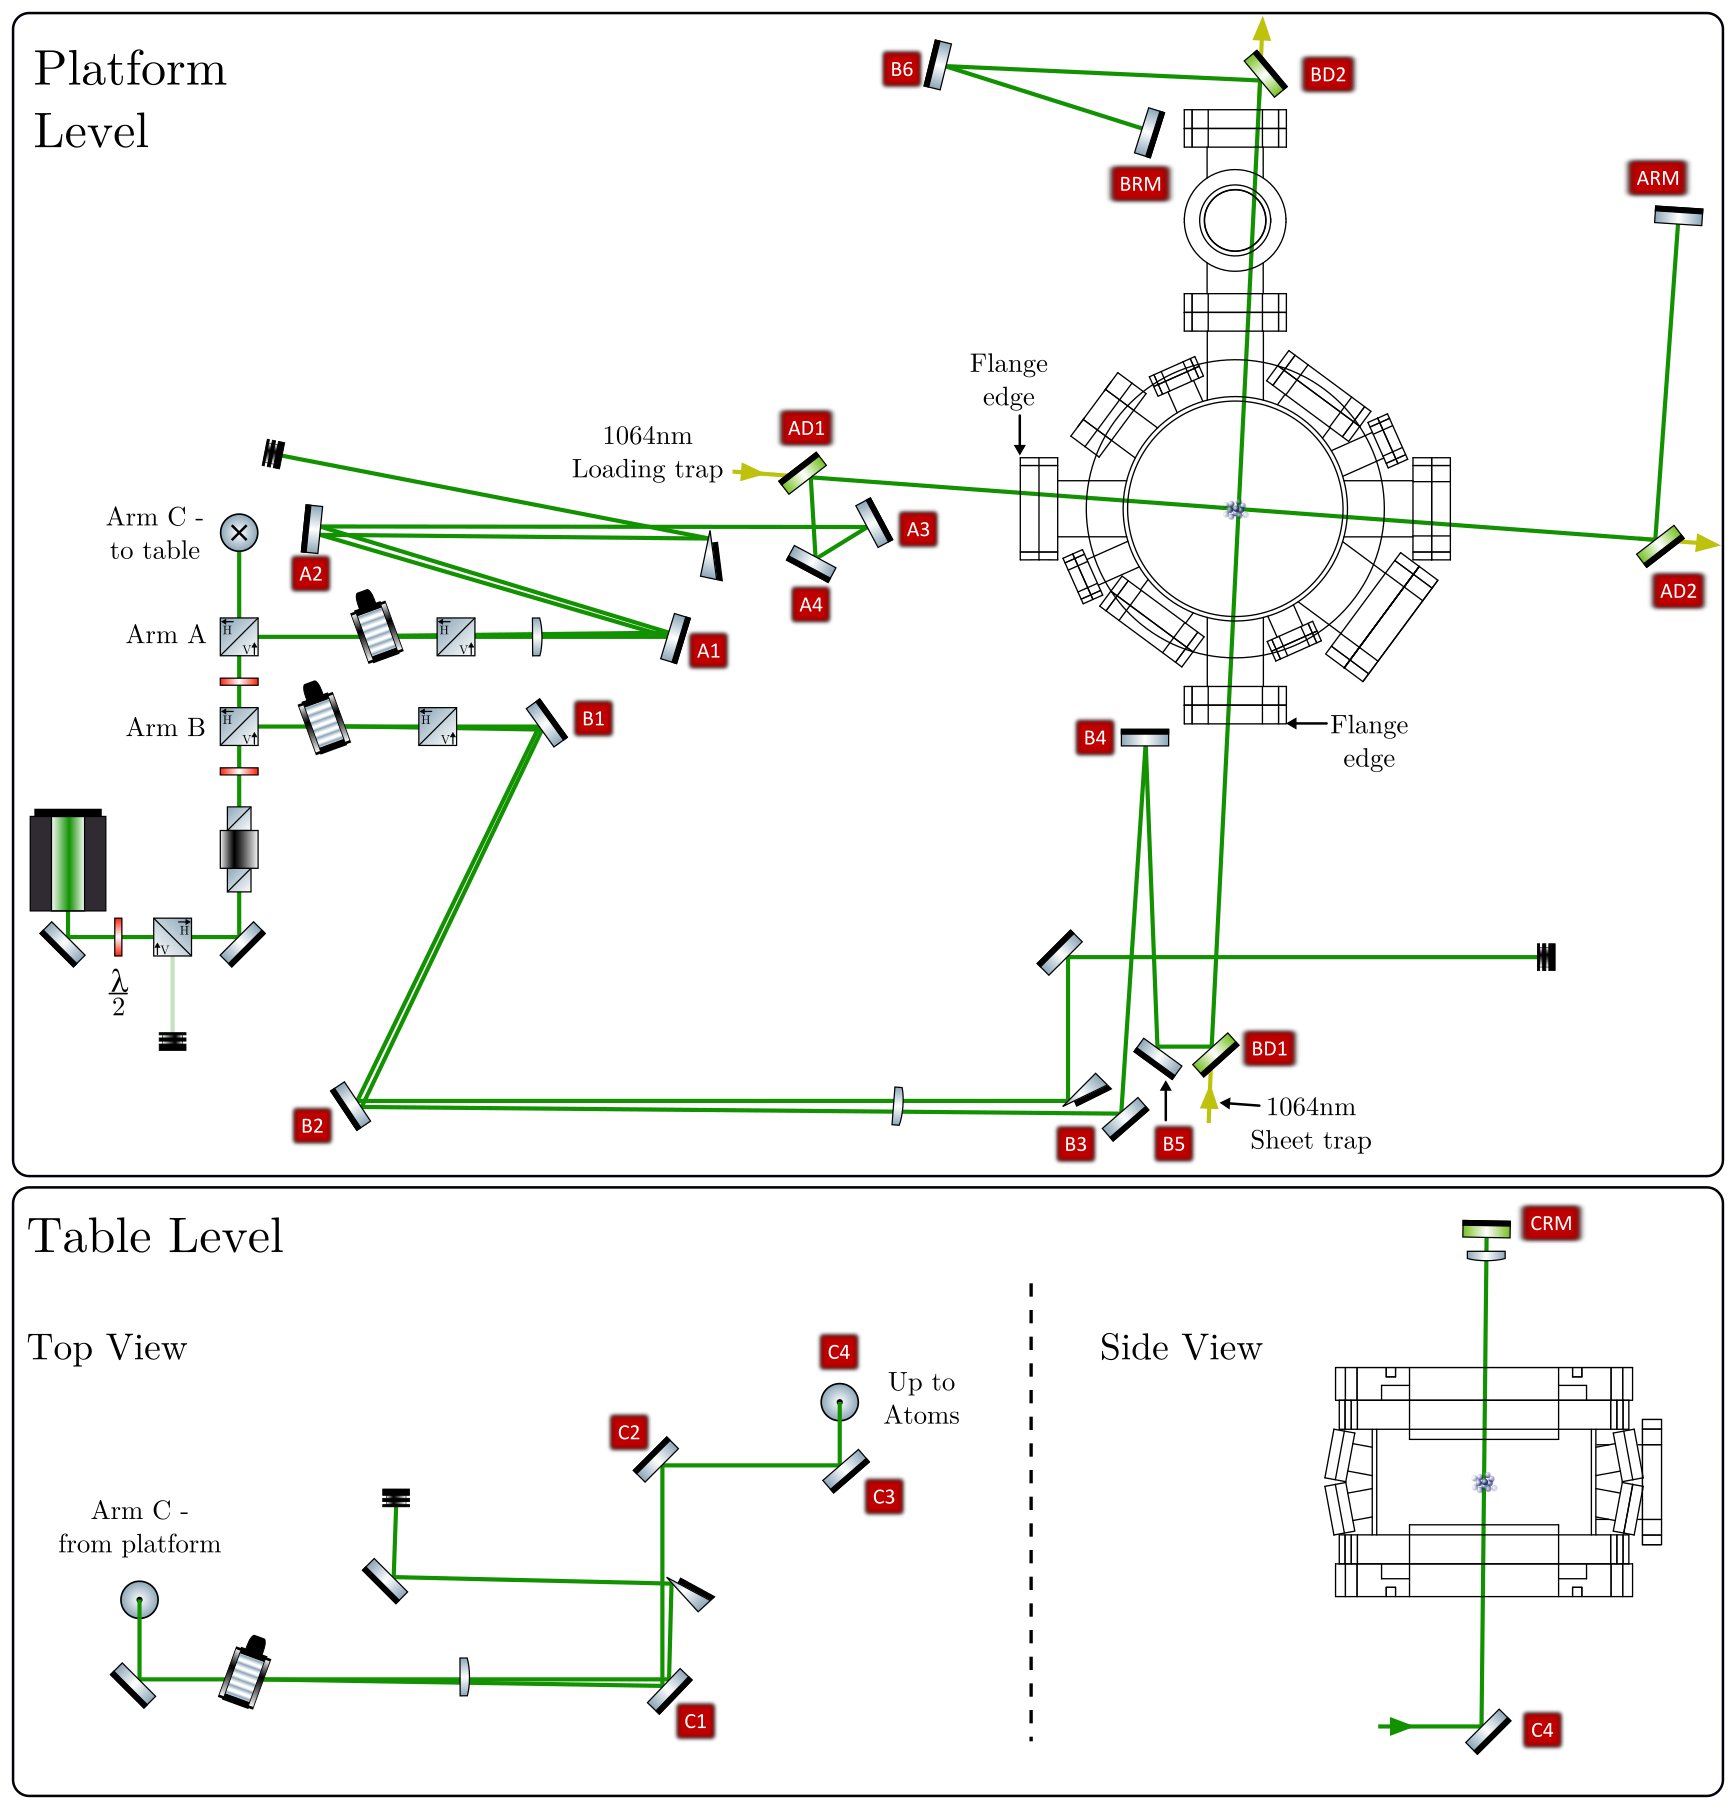
\includegraphics[width=1.2\textwidth]{lattice_schematic.png}}
		\caption{Lattice optical schematic}
		\label{fig:532schematic}
	\end{figure}
	
	\begin{figure} 
		\centerline{
		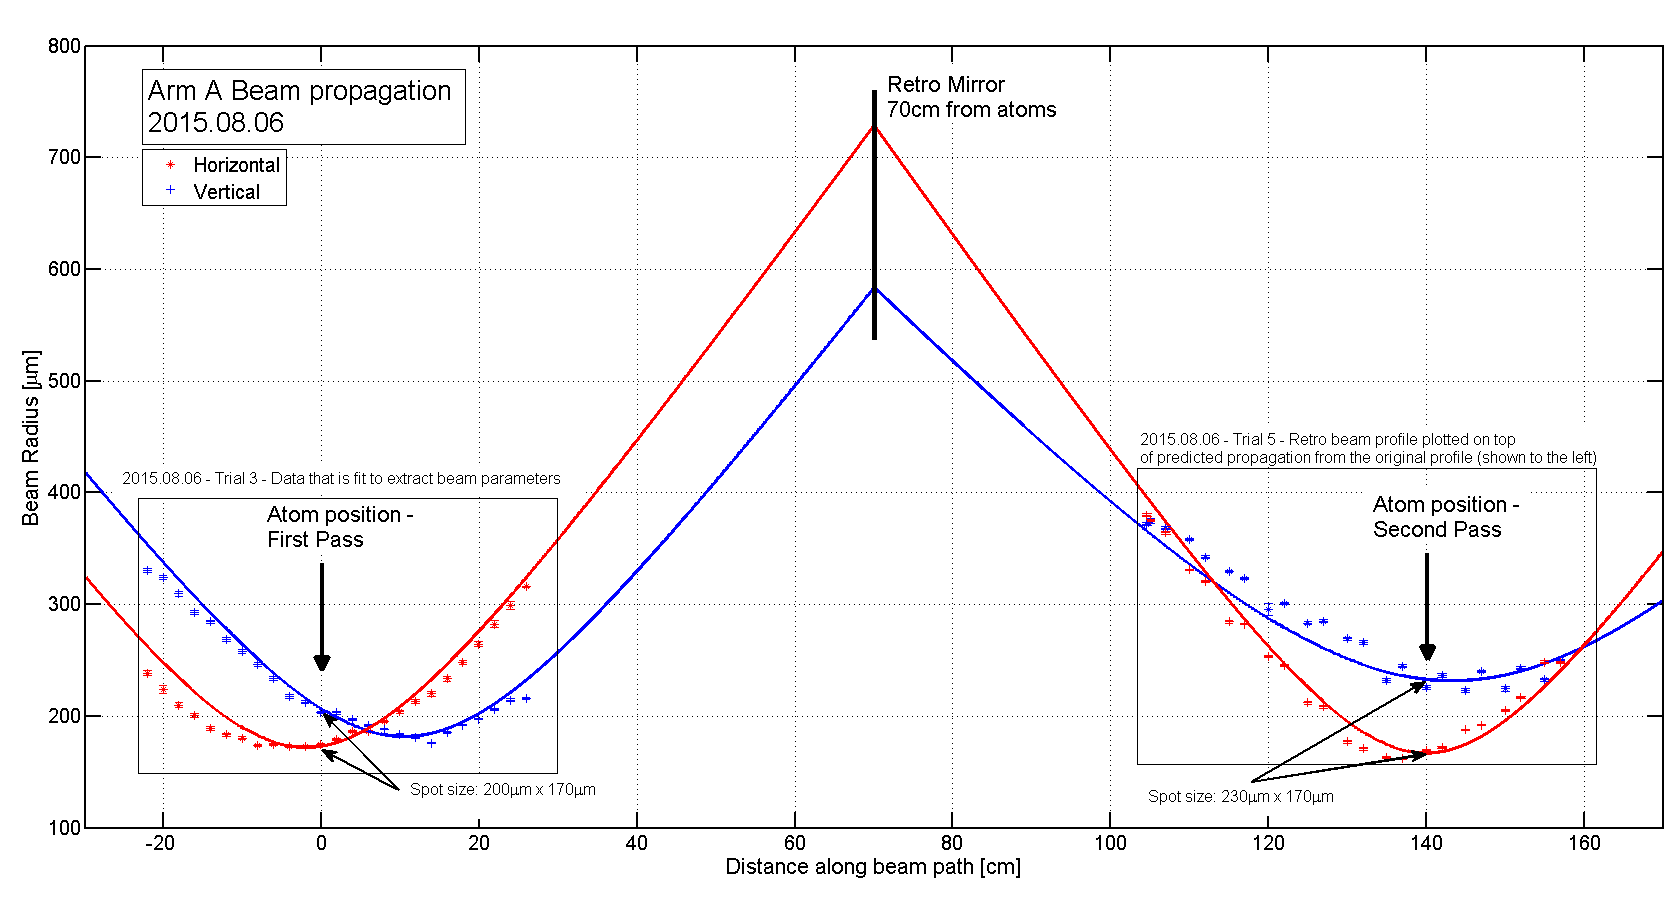
\includegraphics[width=\textwidth]{lattice_ArmAFull.png}}
		\caption{Lattice Arm A profile}
		\label{fig:532armAProfile}
	\end{figure}
	
	\begin{figure} 
		\centerline{
		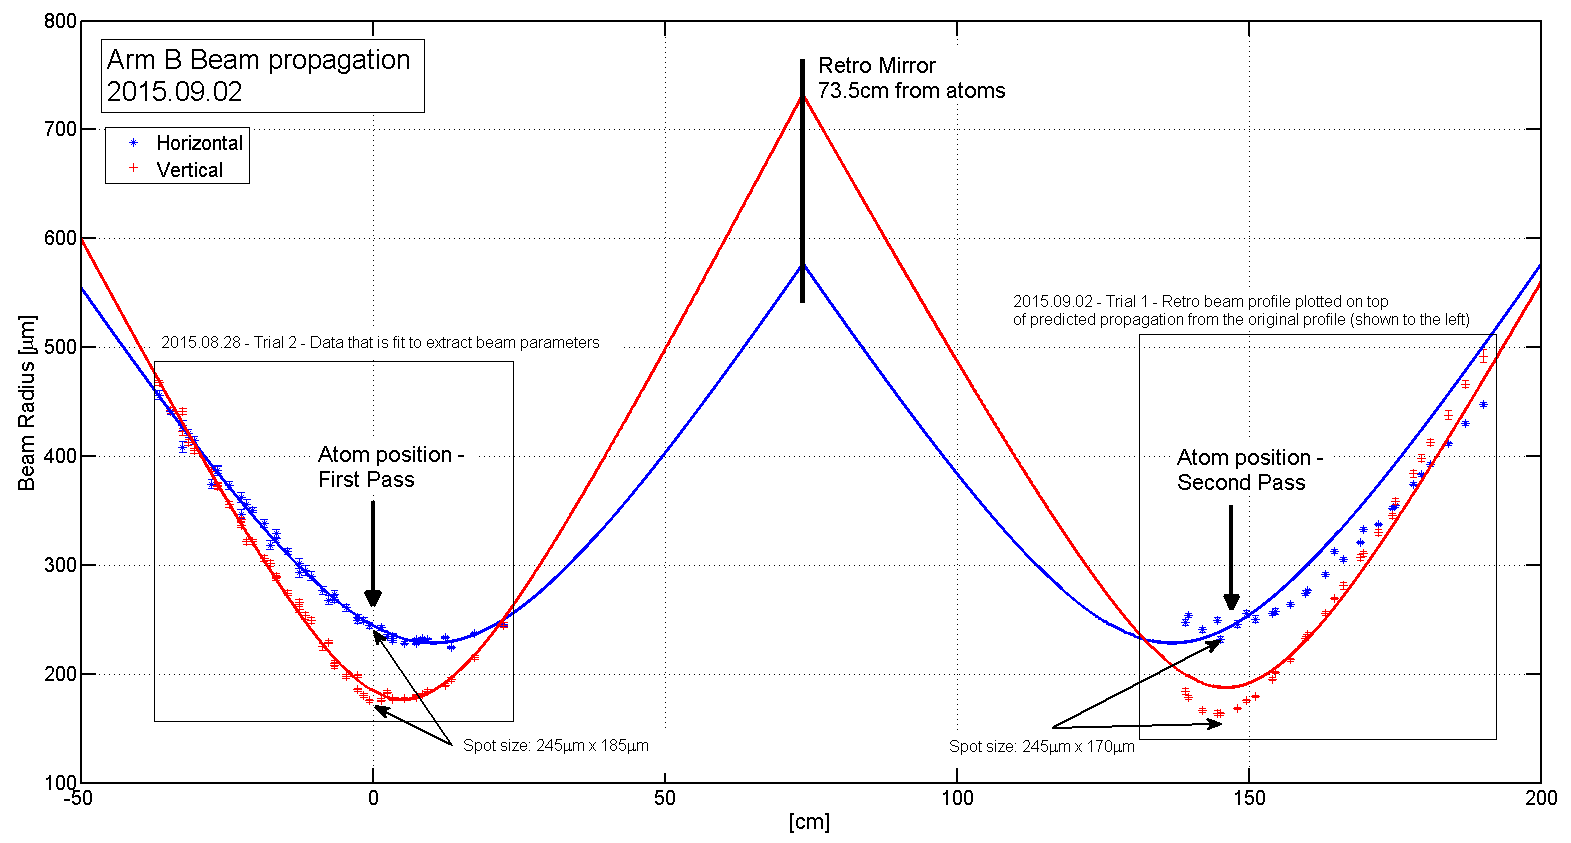
\includegraphics[width=\textwidth]{lattice_ArmBFull.png}}
		\caption{Lattice Arm B profile}
		\label{fig:532armBProfile}
	\end{figure}
	
	\begin{figure} 
		\centerline{
		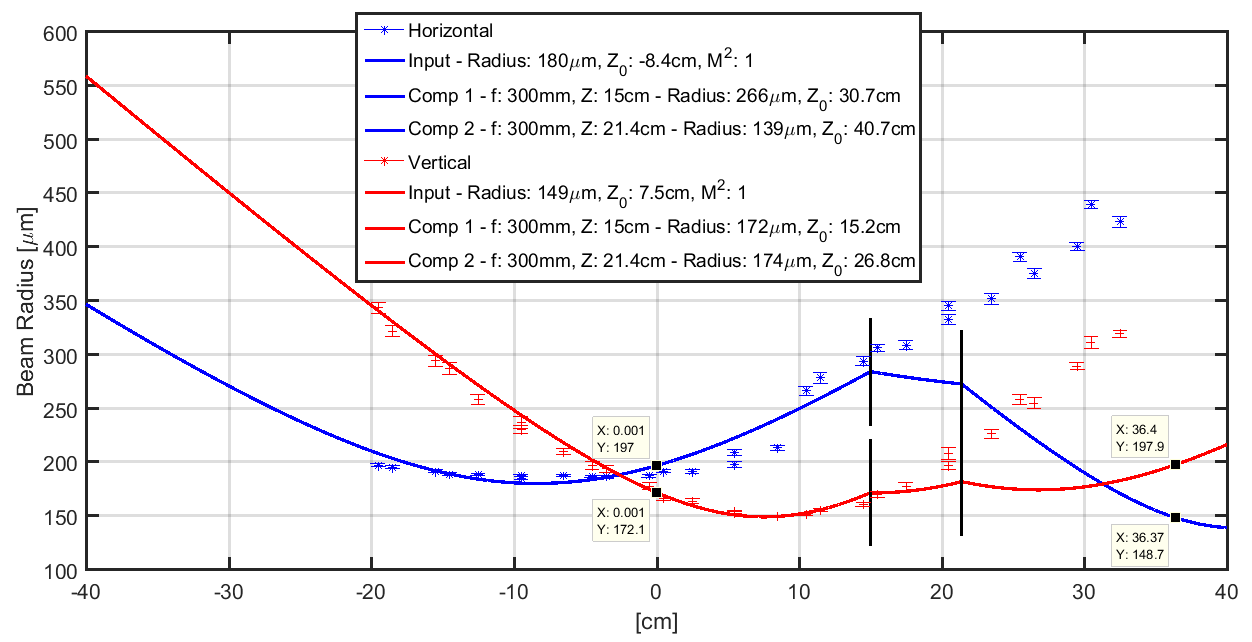
\includegraphics[width=\textwidth]{lattice_ArmCFull.png}}
		\caption{Lattice Arm C profile}
		\label{fig:532armCProfile}
	\end{figure}

\paragraph{Aligning the first pass:}
The following is a technique conveyed to our lab from Trey Porto.
We have successfully used this technique to reproducibly align the first pass of the optical lattice to maximize overlap with the 1064\,nm optical dipole trap.
This process relies on co-locating the trapping regions of the 532\,nm and 1064\,nm traps by observing the change in amplitude of center-of-mass oscillations due to misalignment of 532\,nm 
%misalignment on the equilibrium position of the atomic cloud in the 1064\,nm ODT.
%When aligning, we use the 532\,nm light to cause a sudden shift in the trap minimum position, and thereby induce center-of-mass (COM) oscillation around the new minimum.
%These center-of-mass (COM) oscillations are distinct from breathing mode oscillations where the center-of-mass stays fixed and the atomic density expands and contracts about this point. 
%Breathing modes occur when the atoms are released from the lattice (though still confined to the ODT) and the change in potential depth causes the atoms to pick up energy/velocity and oscillate.
Additionally, we have observed breathing mode oscillations when the 532\,nm and 1064\,nm traps are well overlapped due to the change in trap depth, and correspondingly the potential energy of the atoms, when flashing off the 532\,nm light.

Below is our prescription for overlapping the first pass of the lattice with the IR trap.
\begin{outline}[enumerate]
\1 This process requires the oscillations start from a consistent equilibrium.
We achieve this through the following experimental sequence:
	\2 Typical trapping sequence of blue MOT, repump, red MOT broadband, red MOT single frequency + ODT load
	\2 After loading the ODT, evaporate to a reasonable depth for the given loading time.
	Note that we have observed thermal effects from the ODT which may lead to inconsistent spatial behavior.
	Therefore, the point where the beam overlap should be optimized is at or near the desired IR trap depth for the proposed experiments.
	\2 Following the forced evaporation, hold in the 1064\,nm trap while ramping up the lattice arm being studied to full power.
	We generally find a ramp of $\sim$200 - 300\,ms worked best for strontium 84. 
	\2 Once the green is at full power, we additionally hold for $\sim$250\,ms in the combined 532 + Crossed IR ODT trap to allow for the equilibration of the atoms in the modified trapping potential.
	\2 After the 250\,ms hold, the green is flashed off to excite an oscillation within the IR ODT.
	\2 Image the cloud as it oscillates
\1 To evaluate the procedure above, first focus on in-situ images of the cloud, where atoms are held in the combined 1064 + 532\,nm trap\footnote{
Start by moving the VI cursor positions to be on the cloud center and drawing a box around the cloud location.
This will help to identify small movements of the cloud as well as recording your start position.}.  
\1 When turning off the lattice and allowing the cloud to oscillate, identify the 1/4th period time of the oscillation. 
This is the point of maximum displacement and provides the most sensitive probe for observing how changes to the alignment may vary the oscillation amplitude.
As the alignment is improved the maximum displacement is minimized, this is the signature of improving the overlap.
If unsure about the oscillation period, vary the evolution time after extinguishing the 532\,nm and observe the dynamics of the cloud to resolve a full oscillation.
\1 Each lattice arm (A,B,C) can then be varied along both dimensions (horizontal and vertical) while monitoring the oscillation amplitude. 
Lower amplitude indicates better alignment, but one must be extremely careful, as it is possible to obtain a flat response of the oscillation amplitude when severely misaligned.
We have found that around the minimum in the oscillation amplitude, we are able to flip the phase of the 1/4 period oscillation as we move through the minimum.
This phase flip along with the emergence of breathing mode oscillation are robust measures of good overlap between the beams.
\end{outline}

Fig.\,\ref{fig:latFirtPass} shows an example of the above process where for each scan we have varied the beam alignment slightly and can clearly observe a suppression of the oscillation amplitude.
However, extended time series data in this fashion is arduous and we have found similarly effective alignment to result from the single-point measurement as outlined above.
	\begin{figure} 
		\centerline{
		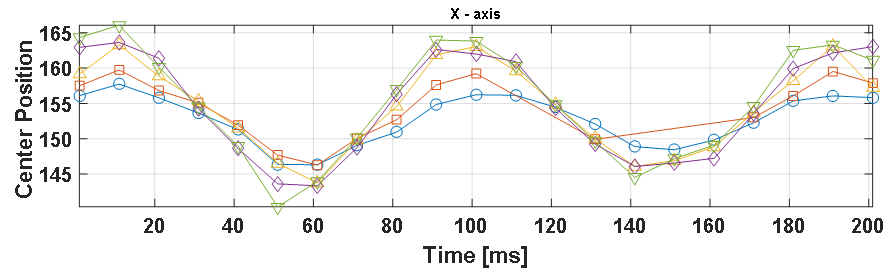
\includegraphics[width=\textwidth]{lattice_first_pass.png}}
		\caption{Center-of-mass amplitude suppression when overlapping traps}{Each subsequent scan is a small variation in the pointing of the last mirror directing the 532\,nm light before the chamber. Note that the Y-axis is in arbitrary units.}
		\label{fig:latFirtPass}
	\end{figure}
	
Additionally, Fig.\,\ref{fig:latBreatheMode} shows the emergence of a breathing mode when the traps are well overlapped.
%We see that while there is significant variation in the size of the atomic cloud, the center position stay relatively constant.
Observation of oscillatory behavior of the cloud radius with reduced deviation of the cloud center is a robust measure of the overlap of the 532 and 1064 traps.
%We note the reproduciblity of the  over a short time period, $\sim$20 minutes, over the complete timescale of these
%We have not found day to day variation in alignment to be a significant source of  but further work remains to ascertain the long term stability of the trap overlap.
	\begin{figure} 
		\centerline{
		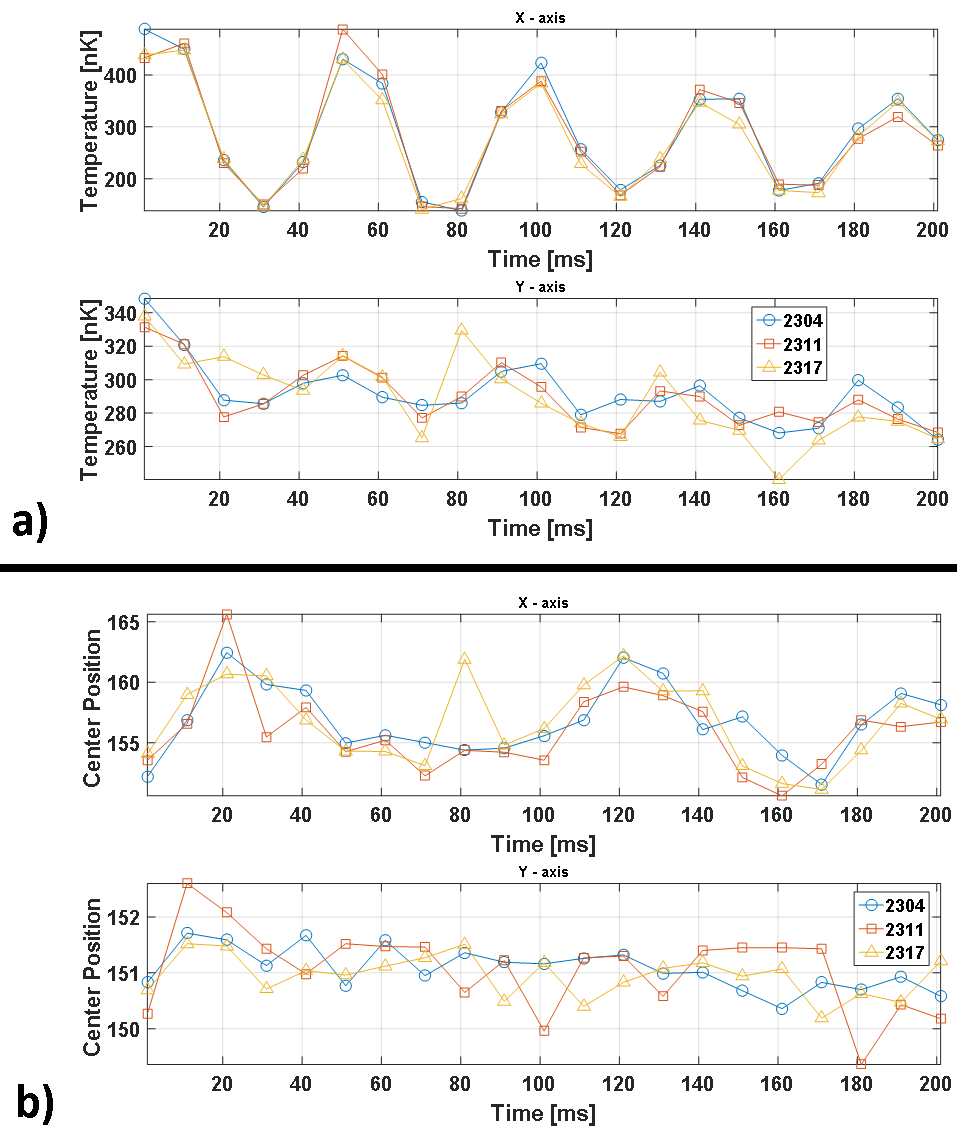
\includegraphics[width=\textwidth]{lattice_BreatheMode.png}}
		\caption{Observation of breathing mode oscillation}{a) The measured radius and b) the cloud center deviation along the horizontal axis.}
		\label{fig:latBreatheMode}
	\end{figure}
	
%\subparagraph{Arm C:} \label{p:armCFirstPas}
%Alignment of arm C 
%The vertical path is special in all this.
%We installed a special mirror as one of the last turning mirrors (give mode).
%We have recently used this mirror to controllable pull the atom cloud in the 1064\,nm for performing trap oscillation measurements as outlined in Sec.\,\ref{ssec:1064sys}.
%Describe using the separate program and it's limitations.
%It is difficult to know we the beam is moving orthogonal to the IR beams but preliminary investigations show that small movements of the mirror axes couple predominantly along the independent IR arms.
%This was deduced by performing a qualitative single point in time two-dimensional search where the in-situ cloud position was observed as the mirror position was varied.
%A more quantitatively rigorous might be able to reveal the coupling between mirror axis by studying the time-series variation of the cloud center at each point of a two-dimensional mirror axis scan.


\paragraph{Aligning the retro-reflection:}
The retro-reflection is optimized via the 2-band Kapitza-Dirac method.
For a quantum degenerate gas in shallow lattice depths, <10\,E$_r$, only the $\pm$1 plane waves will be populated.
Furthermore, for short pulses the amplitude of the population in these plane waves is linearly increasing with lattice depth.
This provides a simple single point measurement which can be used for optimizing the lattice depth.
However, an iterative approach may be needed to ensure that the alignment is only optimized during the first quarter period before the population of the orders is maximized.
Fig.\,\ref{fig:KDoscillations} shows an example oscillation.

As our lattice is free space, the first order alignment of the retro-reflection is to overlap the incoming and retro-reflected beam over a long distance.
This tends to overlap the two beams closely enough in the region of the atoms so as to begin observing diffraction effects when performing a short high intensity pulse of the 532\,nm light.

Second, once we can observe diffraction, the gimbal mounted retro mirrors are adjusted to maximize the population of the diffracted plane waves\footnote{This alignment is extremely sensitive and may ultimately benefit from a more reproducible method of adjustment as mount backlash can strongly effect this process.}.
As the diffracted population is oscillatory and depends on laser intensity we have found that using an exposure time of approximately 2 - 3\,$\mu$s and varying the laser intensity has led to the most successful alignments of the retro.
We generally start with this short time pulse of a few microseconds using the highest intensity pulse possible and systematically decrease the laser power into the lattice arm as the alignment is improved.
Finally we note that, as Kapitza-Dirac happens on very short timescales, the power stabilization circuits must be bypassed for this procedure.
Instead, we directly drive the RF sources with fast analog IC switches (switching time on the order of 10's ns) to apply the desired power to the lattice arm.

\subsubsection{Measurement and results}
\paragraph{Kaptiza-Dirac Scattering}
Kapitza-Dirac diffraction can be viewed as a diabatic projection from an initial eigenstate to a new set of eigenstates which results in an oscillation of the wavefunctions probability amplitudes over the new eigenstates of the system \cite{Denschlag2002}.
As was discusses in Sec.\;\ref{sec:latBackground}, the free space eigenstates are not the eigenstates of the lattice Hamiltonian. 
Thus a pure $p=0$ plane wave, $\ket{\phi_{p=0}}$, suddenly loaded into an optical lattice can be written as a superposition of the Bloch states given by Eq.\;\ref{eq:blochFunc}, here denoted by \ket{n,q}.
	\begin{equation} \label{eq:p0inBloch}
		\ket{\Psi(t=0)} = \sum_{n=0}^{\infty} \ket{n,q} \innerProd{n,q}{\phi_{p=0}}
	\end{equation}
The time evolution of this state is then given by
	\begin{equation} \label{eq:KDtime}
		\ket{\Psi(t)} = \sum_{n=0}^{\infty} \ket{n,q} \innerProd{n,q}{\phi_{p=0}} exp \left( \frac{-i E_n(q) t}{\hbar} \right)
	\end{equation}
where $E_n(q)$ is the energy of the Bloch state at a specified $q$ and $n$ shown in Fig.\;\ref{fig:bandStructure}.
The exponential factor of Eq.\;\ref{eq:KDtime} introduces oscillations among Bloch states and after a second diabatic projection back to the plane wave basis, we can relate evolution of plane wave population to the bandgap energy.
From this analysis we find that for relatively weak lattices, $V_{lat} \lesssim 10 E_r$, the plane wave population will vary as $\omega_{osc} = (E_2 - E_0) / \hbar$.
Where $E_i$ is the band energy of the i$^{th}$ band with $q=0$ as is the case when performing Kapitza-Dirac with a Bose-Einstein condensate.

Fig.\;\ref{fig:KDoscillations} shows a typical Kapitza-Dirac oscillation pattern which we use to maximize beam overlap near the atoms and calibrate our achievable lattice depths. 
Kapitza-Dirac is useful as an alignment tool since measurement of the population oscillation frequency can be highly accurate and directly relates to the bandgap energy in the lattice, shown in Fig.\;\ref{fig:bandStructure}. 
	\begin{figure}
		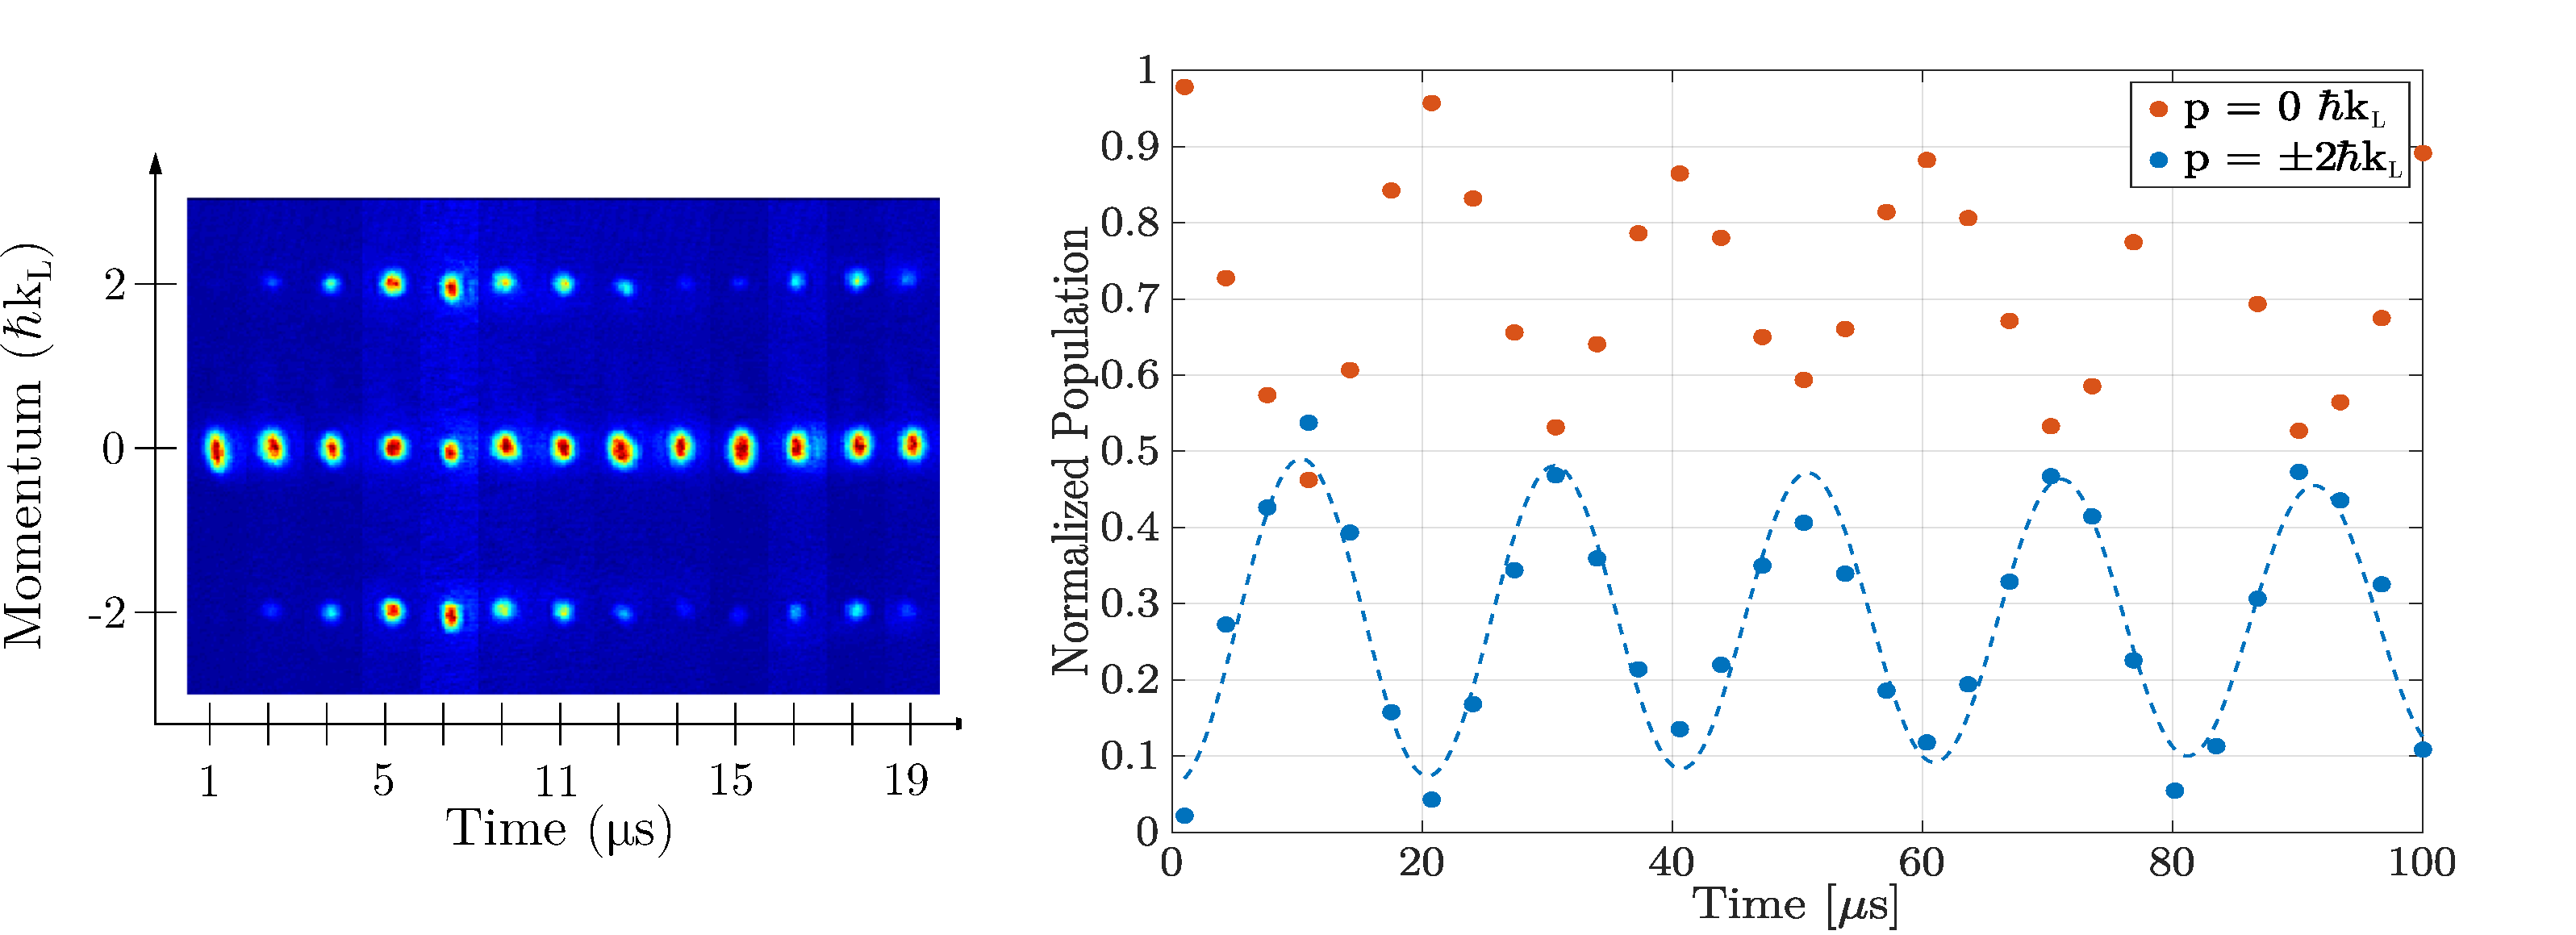
\includegraphics[width=\textwidth]{lattice_kdOsc.pdf}
		\caption{Evolution of plane wave population using Kapitza-Dirac}{Left: Time of flight slices for several realizations of Kapitza-Dirac with varying hold time in the lattice. Right: Normalized population from fits of time-of-flight images. Oscillations are fit with a decaying sinusoidal and the best-fit frequency is used to determine the lattice depth.}
		 \label{fig:KDoscillations}
	\end{figure}
	
	\begin{figure}
		\centerline{
		\includegraphics[height=0.4\textheight]{lattice_1DOscPeriod.png}}
		\caption{Oscillation period between $n=0\,\rightarrow\,n=2$ band at $q=0$}{Calculated for a 532\,nm lattice acting on strontium-84.}
		\label{fig:latOscPeriod}
	\end{figure} 
For reference, Fig.\,\ref{fig:latDepth} shows the resulting lattice depth calibration for our most recent alignment.
	\begin{figure} 
		\centerline{
		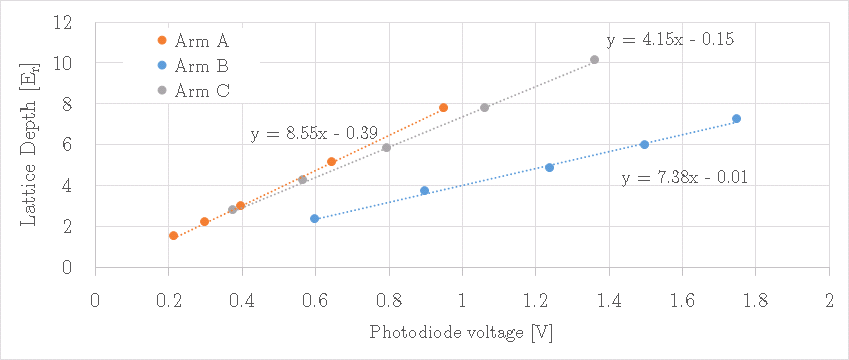
\includegraphics[width=\textwidth]{lattice_depth.png}}
		\caption{Lattice depth calibration}{Calibration was performed using the two-band Kapitza-Dirac technique. Maximum photodiode voltage for each arm is 10\,V}
		\label{fig:latDepth}
	\end{figure}
	
\subparagraph{Higher order Kapitza-Dirac:}
The simple two-band model is a straightforward method for determining the lattice depth but one that requires a time-series measurement over varying lattice depths.
Gadway et. al. \cite{Gadway2009} derived a complimentary depth calibration method which requires only a single time-series measurement at high lattice depth.
This process relies on the quantum interference of the oscillating populations which produces a complex beat note.
An undergraduate report from Alex Wikner \cite{Wikner2017}, follows the original Gadway construction to develop an algorithm using Matlab$^{TM}$ for applying this technique to the Neutral apparatus.
The cited report provides sample code as well as benchmark calculations for comparison.
However, application of this work to calibrate the lattice depth has been stymied by a consistent heating concern we have observed when applying the lattice beams for significant periods at high lattice depths.

\paragraph{Heating of a quantum degenerate gas}
While Kapitza-Dirac diffraction is useful as a characterization tool, we typically wish to maintain equilibrium when loading condensates into the lattice. 
Thus slowly ramping up the lattice laser intensity will adiabatically transform a plane wave ground state into the ground Bloch state of the lattice \cite{Sakurai2010}. 
Strictly speaking, in order to adiabatically connect the free space eigenstates and the lattice eigensates, the lattice must be turned on infinitely slowly due to the infinitesimal bandgaps which open near the band edges. 
Although near the band center, $q=0$, the adiabaticity requirement relaxes to $dV_{lat}/dt \ll 16E_r^2/ \hbar$, \cite{Denschlag2002} which for strontium in a 532\,nm lattice is $\approx 5\,\mu$s$/E_r$. However, in practice we find that our condensate fraction is reduced during fast ramps into the lattice. 
Instead, we slowly ramp on the lattice over 100\,ms which reduces heating caused by the ramp. 
We have experimented with various functional forms of this pulse shape and currently rely on an S-shaped curve given by Eq.\,\ref{eq:sCurve}
\begin{equation} \label{eq:sCurve}
	V_{sCurve}(A,B,C,t) = \frac{A-C}{2} \left[ \, \tanh (2 \pi B[t-1])+1 \, \right] + C
\end{equation}
where A is the overall amplitude starting from zero, B is the timescale for one period, and C is a constant offset term.

As shown in Fig.\;\ref{fig:heatingRates}, we observe a large condensate fraction after ramping the lattice up and back down in this manner to demonstrate restoration of BEC coherence.
Further characterization of the lattice required us to measure the reduction of atom population over long times due off-resonant light scatter.
For our red detuned optical lattice we expect the off-resonant scattering rate to be well approximated by a simple two level approach. In this model, the effective scattering rate is given by \cite{Jaksch2005}
	\begin{equation} \label{eq:offResScatter}
		\Gamma_{eff} \approx \frac{\Gamma V_{lat}}{\hbar \delta_{lat}}
	\end{equation}
where $\Gamma$ is linewidth of the dipole transition between the two states, $V_{lat}$ is the lattice depth, and $\delta_{lat}$ is the detuning of the optical lattice from the two level transition frequency.
In strontium, the $^1S_0\!\rightarrow\!^1P_1$ transition strongly dominates the polarizability of the ground state and therefore can be used to estimate the effective off-resonant scattering rate.
For this transition $\Gamma = 2 \pi \times 30.5\,$MHz and a 532\,nm lattice is detuned by $\delta_{lat} \approx 2 \pi \times 87\,$THz.
With a lattice depth of $V_{lat}=10\,$E$_r$ we expect a scattering rate of $\Gamma_{eff} \approx 2\e{-1}\,$s$^{-1}$, which is negligible for the timescales of our proposed experiments.
From Fig.\;\ref{fig:heatingRates}, we see that there is not an appreciable loss of atoms over a one second timescale.
	\begin{figure}
	\centerline{
		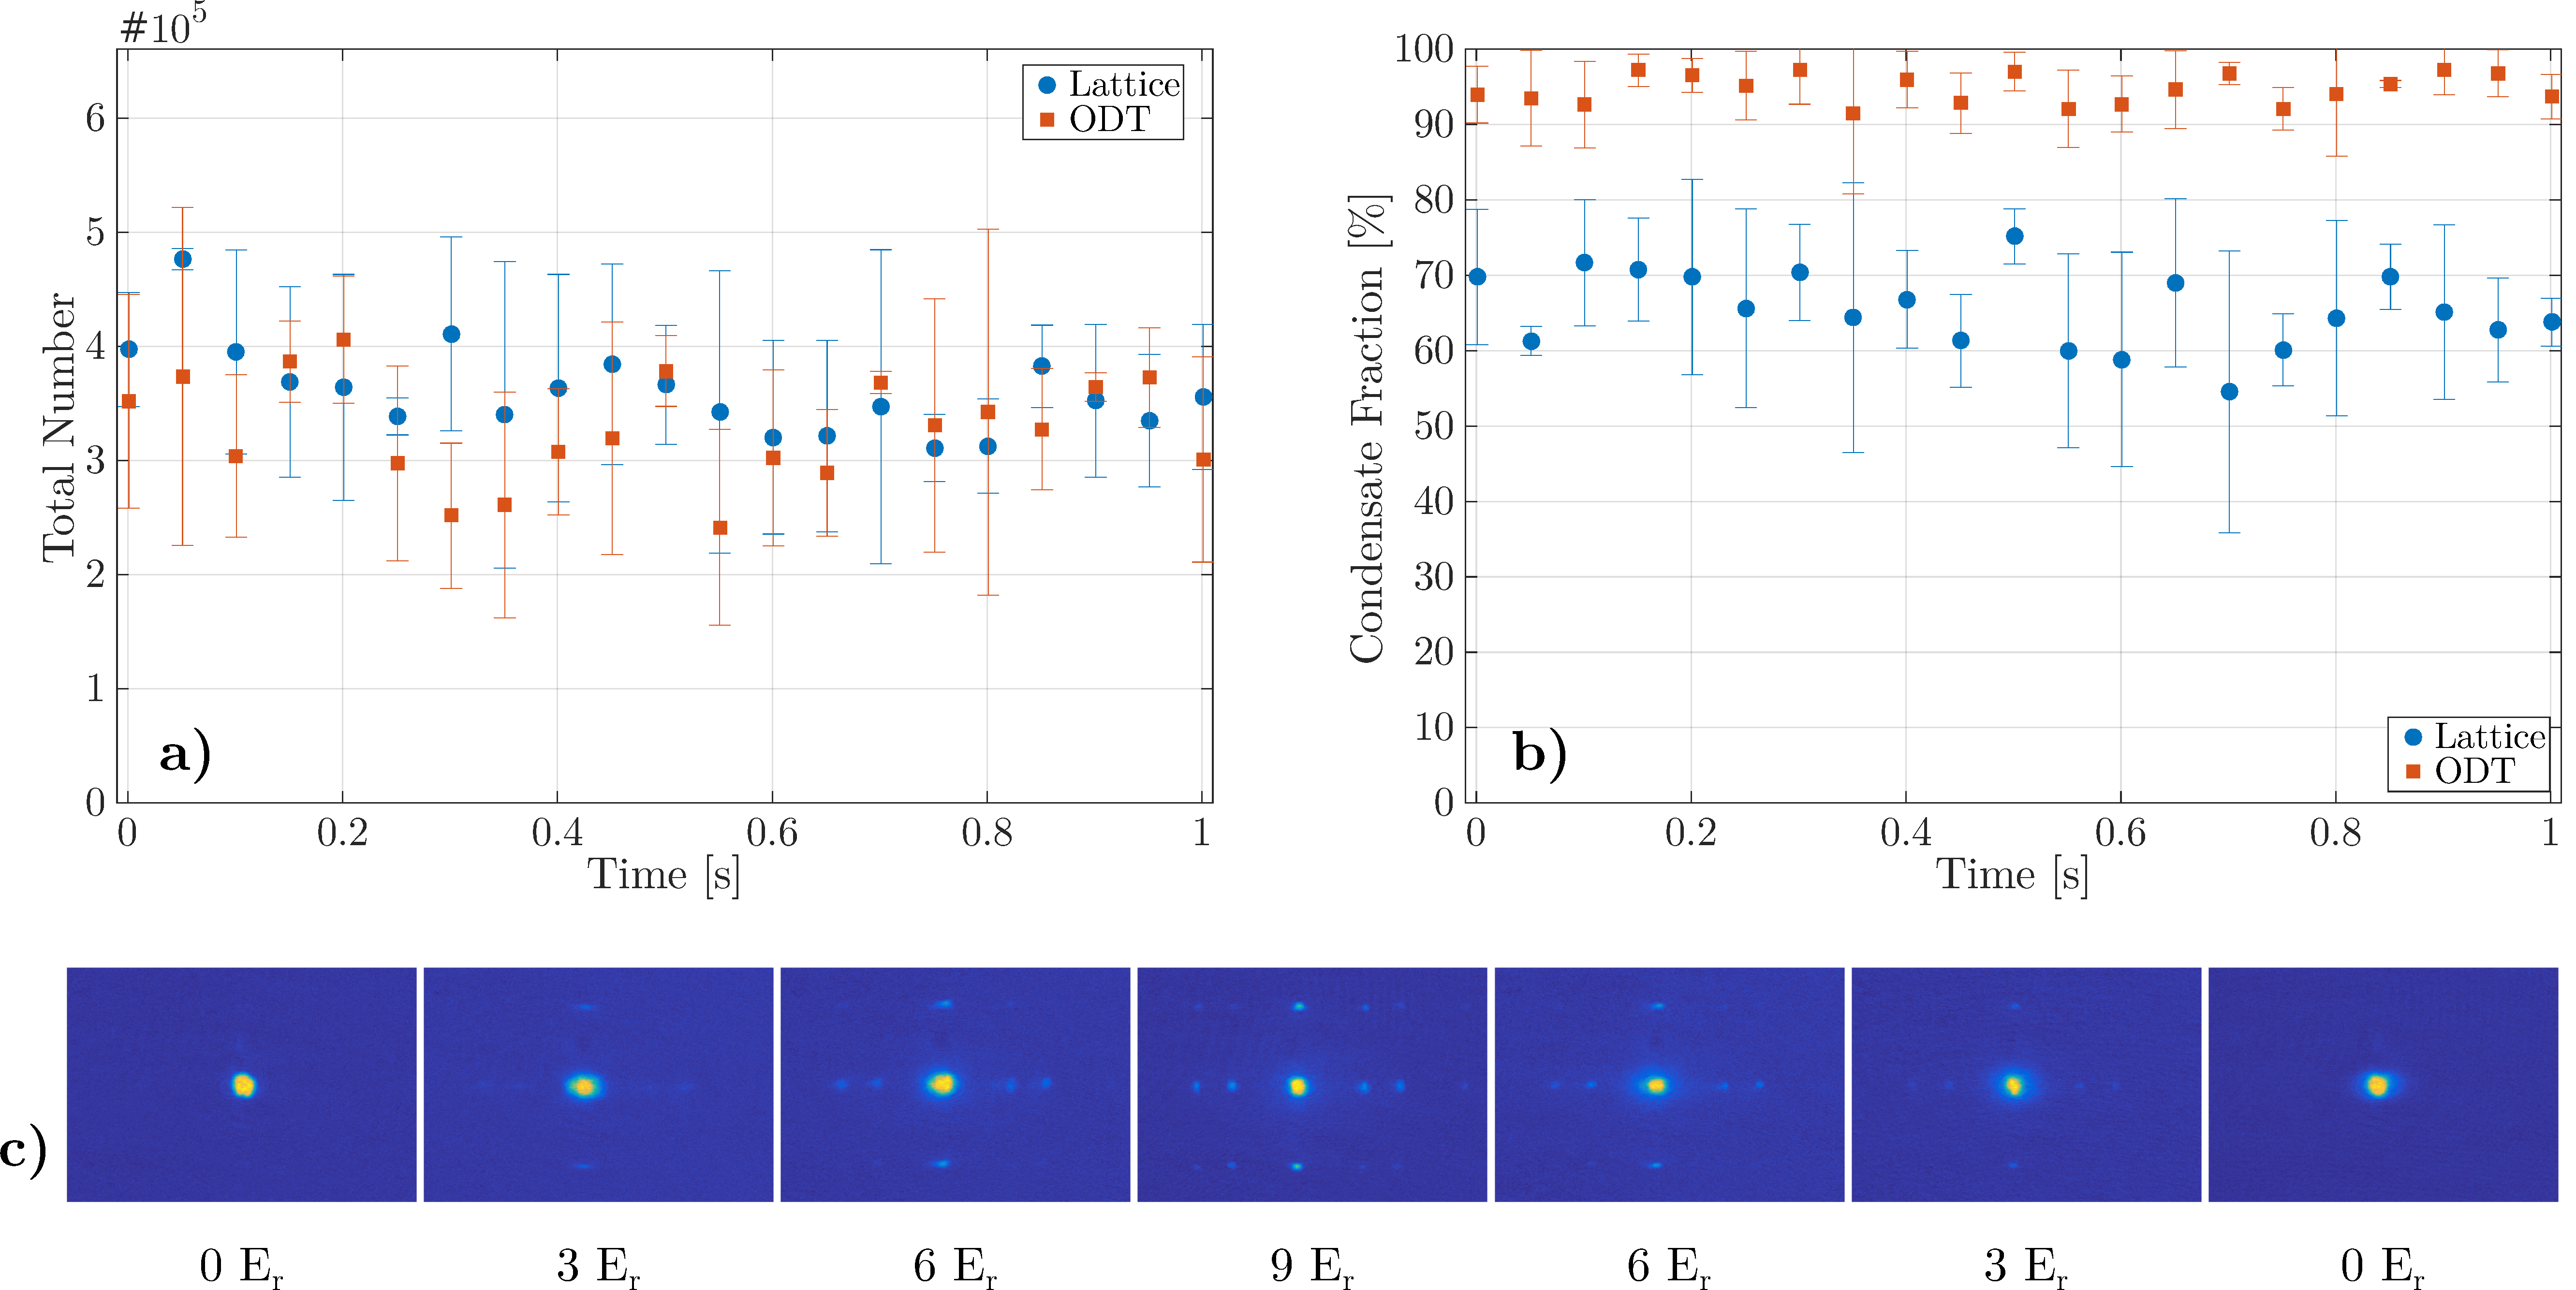
\includegraphics[width=\textwidth]{lattice_heatRates.pdf}}
		\caption{Characterization of heating in the optical lattice}{Evolution of condensate fraction over time after adiabatically ramping on the lattice to 9\,E$_r$. a,b) Comparison of total number and condensate fraction for a sample held in the optical dipole trap (red squares) or in a deep lattice (blue circles). c) Time of flight images after ramping on the lattice and diabatically projecting back to plane wave states.}
		 \label{fig:heatingRates}
	\end{figure}
Unfortunately, we have recently observed that attempts to load a degenerate gas into a deep lattice, $\gtrsim 15$\,E$_r$, and hold over long timescales leads to unacceptable heating of the atomic sample.
Currently, we hypothesize that this may result from the freespace nature of the lattice or an intrinsic instability (frequency or power) of the Verdi.
The latter of these has been tested by monitoring the 532\,nm light in a spectrum analyzer where no obvious deficiencies have been observed.
To test our stability hypothesis, we are currently investigating fiber coupling one of the arms of the lattice but as of spring 2019, this project is ongoing.

\section{Spin manipulation of $^{87}$Sr}
\label{sec:spin_pol}

Here is where I need to introduce and characterize the \hl{LCR}

Averaging images together (how to use this code specifcally)

don't forget to talk about optimizing the polarization of the fixed waveplate

Fig. \hl{something} shows the variation of the retardance angle for 689\,nm light.

For reference, Fig. \ref{fig:mF87} reproduces the Clebsch-Gordan coefficient diagrams originally created by Pascal.
From this diagram we can easily see how optical pumping works.
Let us consider an atom starting in the $m_F=-9/2$ ground state and being exposed to $sigma+$ photons acting on the $F=9/2\,\rightarrow\,F=11/2$ hyperfine transition.
Absorbing a photon promotes the atom to the $F=11/2, m_F=-7/2$ state.
From here we can consult Fig. \ref{fig:mF87} to find the dominate decay path to be to the $F=9/2, m_F=-5/2$ state due to the Clebsch-Gordan coefficients.

Now we have a couple of options, by taking advanatage of the CG coefficents we see that we will probabilitically promote population towards a polarized state.
In the absecene of a bias field the magnetic sub-levels are degenerate so this oculd be an efficeint process.
In practice we find this to heat the atom population significantly.
Therefore, in a bias field, we split out the levels by approx. 200\,kHz to and address each sub-level transition individually.
This allows us to minimize the number of photon scattering events which we hypothesize to be the cause of the observed heating.

can individually address the separate hyperfine sub-level transitions and sequentially pump population towards one a polarized state 
	\begin{figure}
		\centerline{
		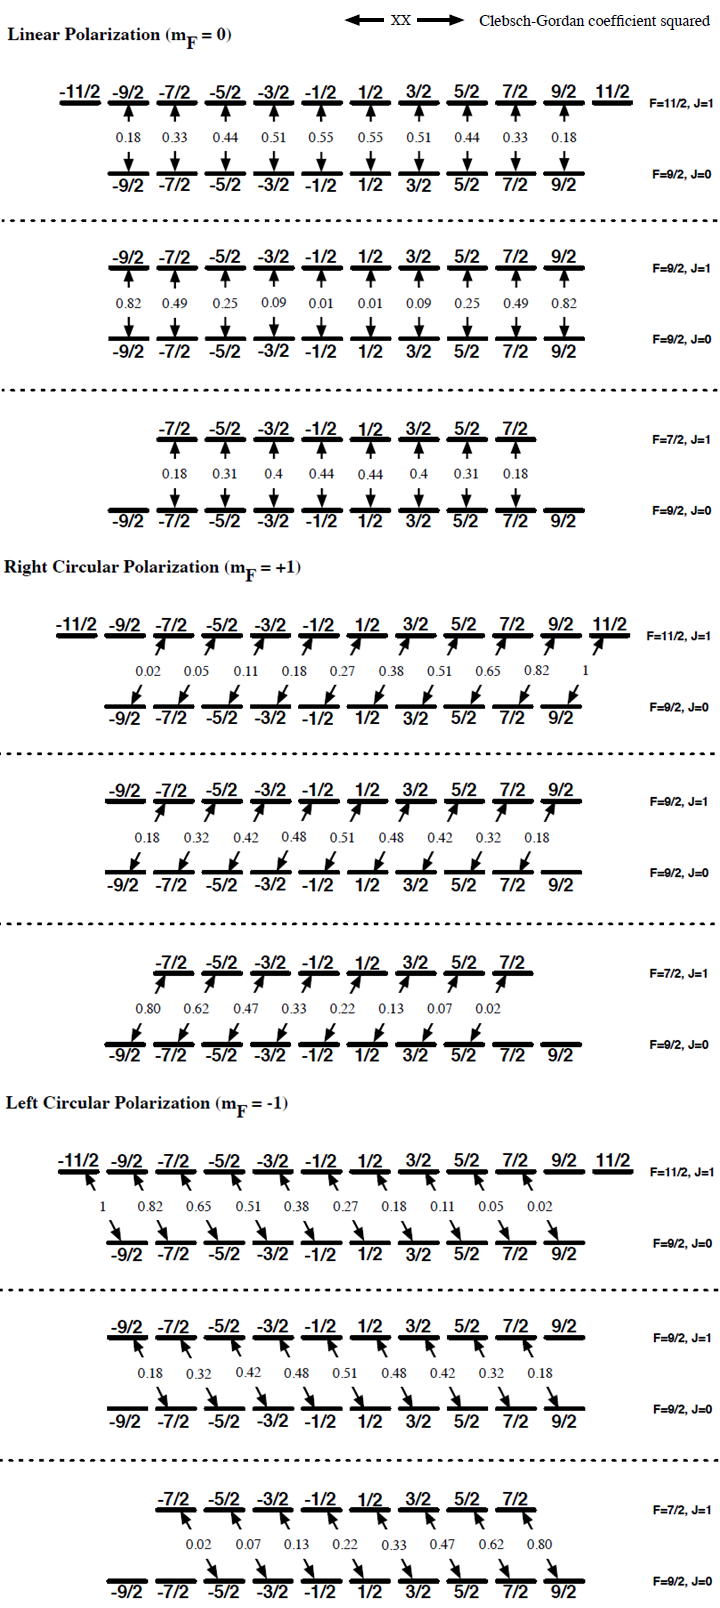
\includegraphics[height=\textheight]{87_CG_coeffs.png}}
		\caption{$^{87}$Sr $^1S_0 \, \rightarrow \, ^3P_1$ hyperfine structure}
		\label{fig:mF87}
	\end{figure} 
	
Be sure to define convention for what we determined was plus and minus

\section{Search for narrowline PA molecules using various spin mixtures}
\label{sec:87PAS}

"Lorem ipsum dolor sit amet, consectetur adipiscing elit, sed do eiusmod tempor incididunt ut labore et dolore magna aliqua. Ut enim ad minim veniam, quis nostrud exercitation ullamco laboris nisi ut aliquip ex ea commodo consequat. Duis aute irure dolor in reprehenderit in voluptate velit esse cillum dolore eu fugiat nulla pariatur. Excepteur sint occaecat cupidatat non proident, sunt in culpa qui officia deserunt mollit anim id est laborum."
